%% M3 Challenge Report Document
%% To add a source, use bibme.org/bibtex to generate a bibtex format citation and paste it into main.bib under the other citations then recompile the document.
%% To reference it in the text use \cite{NAME PLACED INSIDE BRACKETS IN BIB FILE e.g. DUMMY:1}. This ensures that if you create a new reference that comes before it, the reference numbers update automatically.

%% Any lines starting with a % sign are ignored and can be used to write a comment, or you can use the speech bubble to the left. Make use of this feature as it is something you can't do in Google Docs so it validates use of LaTeX ;)
%% Please check your work by activating the spellchecker in the top right corner. Simply select English and then when a word is underlined, click it and press Alt-Enter to see suggestions.

%% Acceptable to research existing models as long as additional insight is provided on top of them
%% If possible try to preserve indentation - after every begin{} there should be an extra tab on the new line and remove a tab after every end. You can tab a bunch of lines in one go by highlighting and pressing tab.

% Judges will be considering the following Discretionary Points
%   Team examined a wider set of circumstances.
%   Team used a creative problem solving perspective.
%   Team made connections between all three parts and the overall driving question.
%   Paper is exceptionally well written/organized.
%   Detailed sensitivity analysis is presented.
%   Model verification is performed.
%   Strengths and weaknesses are addressed.
%   Effective and well-motivated use of technical computing


% Please check: https://m3challenge.siam.org/sites/default/files/uploads/M3%20Challenge_Scoring%20Guide_generic-FINAL13SEPT2021.pdf
% Technical Computing Award. Solutions that receive the award must demonstrate an outstanding use of computing to advance the team’s model or to reveal its implications (including via advanced model and data visualization).

% Page limit is 20 pages not including the Appendix
% May need to rethink the use of \newpage command if too many pages. Do that at the end

%CHECKERS OF THE REPORT:
% Points to check through at the end:
    % Are all figures and tables captioned and numbered, and then referenced later in the text?
    % Spelling and grammar (use spellchecker in the top right)
    % Excluding the appendix, is the report less than or equal to 20 pages?
    % Have we removed any dummy/template text such as the dummy citation in the bibliography and the template code at the bottom to avoid any loss of professionalism?
    % Are units given to all variables?
    % Every single assumption must be justified (make up a justification which sounds legit if necessary)
    % Are all sections completed including conclusion etc.?
    % Are there any numerical typos (numbers which look wrong)?
    % Are all models analysed in terms of their strengths and weaknesses? 
    % Are all sources cited?
    % When a source is cited have we made it clear exactly what tables / data / ideas etc. were used from that source?
    % When code is used, have we made sure that it is fully explained / referenced inside the relevant section rather than just being dumped at the bottom with a "check the appendix" comment? - They are big on saying that "the code is not a model; the theory behind the code is". Therefore it's important that all algorithms are well explained. If necessary resort to a flowchart.
    % Are there any coding mistakes/typos
    % A comment we received last year: " The model on the whole would have benefited greatly from some data validation." - do we see any points in the model where we could add a sentence or two to explain what we did to validate the input or output data for the model? i.e. are we performing sufficient model analysis?
    % Check all headings and subheadings are correct based on the content of the section and that none have been missed out.
    % Look for any references that don't work right. these come up as ?? in the pdf.

\documentclass{mthree}

\author{Team 15440} % ****Provide only your team ID #. Do NOT include your school name, any student names, or any other identifying information in your solution paper.
\title{Remote Work: \textit{Fad or Future?}}
\date{February 26, 2022}

\usepackage{booktabs} % For prettier tables
\usepackage{graphicx} % To enable images to be inserted
\usepackage{float}
\usepackage{enumitem}
\usepackage{amsmath}
%\usepackage{hyperref}

\graphicspath{ {images/} }

\setlist[enumerate,2]{label*=\arabic*.}


\begin{document}
    \maketitle \thispagestyle{fancy}

    
    \section{Executive Summary}
        % not more than one page in length.
        % This is one of the most important parts of the document as judges "will not read past a poorly written summary"
        % Reserve 1 hour for one person just for writing and perfecting this at the end of the time.
        % P1 : Context, motivation, general problem overview. Challenge associated with the problem context - why is it difficult? Motivations. Spark curiosity and make the reader eager to see what you did. Why is the problem important? Does part 1 indicate that part 2 is important for example? CITE SOURCES TO FILL UP BIBLIOGRAPHY
        % P2 : Problem Part 1 - overview of the question, your methods (mathematical approaches), your results and what they mean in context in terms of recommendations
        % P3 : Problem Part 2 - overview of the question, your methods  (mathematical approaches), your results and what they mean in context in terms of recommendations
        % P4 : Problem Part 3 - overview of the question, your methods  (mathematical approaches), your results and what they mean in context in terms of recommendations
        % https://m3challenge.siam.org/sites/default/files/uploads/CHAMPION_14817.pdf for reference
        % use \\ to get the new paragraph
        
        %"what we think should be taken away from this model"
        % https://m3challenge.siam.org/sites/default/files/uploads/Team_12038_FINAL.pdf
        
        % executive summary - results and recommendations
        % Overview of the problem (all three parts).
        % Brief description of the mathematical approaches that will be used.
        % Provide and discuss a summary of the results (even if they are incorrect). You do need your results.
        % Recommendations made as a result of the model
        % Start by setting the question in context
        
        % Use big words and make it flow nicely
        % ***Free of technical maths jargon (problem context jargon ok I think)
        % What is the challenge associated with the problem - i.e. why is it difficult?
        % motivations and conclusions
        %Its introduction should spark curiosity and make the reader eager to see what you did. 

        %problem you were solving, methods and conclusions

        % P1 : Context, motivation, general problem overview. Challenge associated with the problem context - why is it difficult? Motivations. Spark curiosity and make the reader eager to see what you did. Why is the problem important? Does part 1 indicate that part 2 is important for example? CITE SOURCES TO FILL UP BIBLIOGRAPHY
        % P2 : Problem Part 1 - overview of the question, your methods (mathematical approaches), your results and what they mean in context in terms of recommendations
        % P3 : Problem Part 2 - overview of the question, your methods  (mathematical approaches), your results and what they mean in context in terms of recommendations
        % P4 : Problem Part 3 - overview of the question, your methods  (mathematical approaches), your results and what they mean in context in terms of recommendations
       
       Nobody could doubt that the global coronavirus pandemic has led to radical shifts in work patterns. According to the ONS \cite{ONS}, the proportion of people working from home increased by a phenomenal 10 percent points from 27\% to 37\% from 2019 to 2020. But even before this, trends towards homeworking were on the rise, from only 22.0\% in the US in 2005 to 25.0\% in 2013. While working from home offers substantial benefits such as an improved work life balance \cite{ONS}, it can lead to reductions in productivity - undesirable for employers.
       \\ \\
       In this paper, our team investigates how the trends towards homeworking can be applied into the future, in a post pandemic society. We apply our models for the percentage of jobs that can be done from home and that \textit{will} be done from home to 5 cities: Scranton (PA), Seattle (WA), Omaha (NE), Liverpool (England), and Barry (Wales), in the hope that this important research can be used to improve sustainable policy making in the US and UK alike.\\
      
       In Part I of the problem, we are asked to determine the percentage of jobs in the 5 given cities. We divide the labour market within each city into 10 main sectors and make use of an exponential regression model to track the relative proportions of each sector in each city's labour market over time. From this and an estimated proportion of jobs in each sector that can be performed remotely, we achieve results of around 40\% of jobs being able to be completed remotely in each of the cities, with the maximum being for Seattle, which we believe to be logical considering Seattle, home of Amazon, is one of the most technological cities\\
       
       In Part II, we are asked to determine for a given worker who can work from home, whether they will actually work from home, considering the likelihood that they want to work from home and that they are allowed to work remotely. Based on a variety of demographic factors, we make use of a model derived from conditional probability to estimate the percentage chance for a given worker that they work from home. This can be compared to the critical value of 0.5 to yield a binary result for a given worker. We give a white male IT Worker aged 40 63\% chance of working from home, for example.  
       \\\\
       In Part III a fusion of the models for jobs (Part I) and for individuals (Part II) in the form of a Monte Carlo simulation is employed based on projected demographics of each town or city to obtain the expected proportion of remote workers. We obtain results ranging from 26.5\% for Barry in 2024 (logical as Barry is not as technologically developed as some regions in the UK, and 2024 is only 2 years away), to 32.5\% for Seattle in 2027.
       \\\\
       As a result, we make the policy recommendation for the Prime Minister that working from home will remain a substantial part of the UK and US work-forces. He must consider it in future labour policies, and the impact of improved technology on the propensity to work from home should be factored into his levelling up agenda. 
      

        
        % https://m3challenge.siam.org/sites/default/files/uploads/CHAMPION_14817.pdf
    
    \newpage %starts a new page, as you may expect.
    \setcounter{tocdepth}{2}
    \tableofcontents
    \newpage
    
    \section{Introduction}    
        In this paper we provide an in-depth analysis of post pandemic working trends in the US and UK, from the proportion of people that are in remote-ready jobs in different towns and cities, to the proportion who will actually take the plunge and leave the office in the near future.
        
    \section{Global Assumptions}
        Throughout this paper we make the following global assumption:

        % All assumptions made in the model must be stated and justified. Do this in the following way:
        % \item creates a new bullet point for the new assumption
        % \assume{The thing you are assuming}{The justification for this assumption}
        % So overall write this: \item \assume{assumption}{justification}
        
        \begin{enumerate}[label={G.\arabic*.}]
            \item \label{G:partialwork} \assume{Working from home is defined as working from home at least 1 day per week.}{We have recently seen a rise in hybrid working models in which working from home occurs one day a week, to complement existing models where you either work from home the whole time or not at all. As the problems generally concern themselves with whether a given person "works from home" or a given job can be done "remotely" we are free to choose whether we include these hybrid models. Their inclusion under an umbrella "work from home" term simplifies the scenario to make it more tractable, without reducing the accuracy of the models too much, since exactly how much a person works from home is much easier to change than going fully from the office to home or vice versa.}  
            % list of possible human(non mathematical) assumptions:

            % there are no major innovations in technology that allow people to work from home more easily.
            %there is no major event that forces people to work from home(ie to force real life business online)
            % no major change in rate of change of population (countries continue to grow at about the present rate)
            
        \end{enumerate}

        
    %To avoid the file getting too large, I have moved the content for each problem out to a separate file, which gets automatically included into this one, using the \input command
    \newpage
    \section{Part I: Ready or Not}
            
        \subsection{Problem Statement}
            % State the problem and describe how you "redefined" it - and also maybe a single sentence before that on why it is important.
            Find the percentage of jobs in the following cities that can be accomplished from home in the years 2024 and 2027:
            \begin{itemize}
                \item[US]
                \begin{itemize}
                    \item Seattle, WA
                    \item Omaha, NE
                    \item Scranton, PA
                \end{itemize}
                \item[UK]
                \begin{itemize}
                    \item Liverpool, England
                    \item Barry, Wales
                \end{itemize}
            \end{itemize}
            
            
        \subsection{Assumptions and Justifications}
            \begin{enumerate}[label={1.\arabic*.}]
                % All assumptions made in the model must be stated and justified. Do this in the following way:
                % \item creates a new bullet point for the new assumption
                % \assume{The thing you are assuming}{The justification for this assumption}
                % So overall write this: \item \assume{assumption}{justification}
                \item \assume{"Work from home readiness" is only dependent on the specifics of the job in an industry and not an employee's own circumstances.}{Employees may not be able to work from home due to their own circumstances, but this will not determine whether the job itself is "work from home ready" or not.}
                \item \assume{Proportion of jobs within a given industry which are "work from home ready" will not change in the near future.}{Any job which is "work from home ready" now, will remain "work from home ready", as there will not be any significant technological advancement in robotics or communication technology which will drastically change how people can work from home between now and 2027.}
                \item \assume{There are no major changes to the trend of industry patterns in a city}{It is reasonable to suppose that there will not be any significant government policy or external effect to change the trend of industry patterns in a city significantly, meaning we can use trends to determine how many people in each city will work in each industry.}
                \item \assume{Every candidate for working from home has a device to work from home.}{Most people in developed countries such as the US and UK own a device and have access to the internet. If someone does not, their employer will likely provide them with a device to work from home}
                \item \assume{After the pandemic, growth in the sectors of the economy we consider will follow pre-pandemic trends, from the lower base of post pandemic levels}{Many employees lost their jobs during the pandemic which brings down the number of jobs in each sector. However, the trends are likely to pick back up to pre-pandemic levels from this point considering that most countries' policies are to return to the previous "normal".}                % USE THE GRADIENT FROM THE NEW VALUES AS THE y icpt.
            \end{enumerate}
      
             
        \subsection{Analysing the Problem}  
            As we stated in our assumptions, the effects of wealth and internet connectivity can be considered negligible on the potential for a job to be done from home as these are independent of the job and can be provided by an employer. Hence, the main important variable in determining if a job is "work from home ready" is the type of job i.e. the industry.
            We have assumed that the proportion of "work from home ready" jobs within a given industry will remain constant ($H_I$) between now and 2027.
            We define an industry pattern to be the proportion of people working in each industry in a specific city at a given time. We start by considering how the industry pattern in a city is changing with time ($P_{I,C}(t)$).
            Using the $P_{I,C}(t)$ function and the $H_I$ constant, we can find the proportion of jobs in a city which are "work from home ready" which we can do by multiplying them together and summing, as follows:
            
            \begin{equation}
                    \sum P_{I,C}(t) \cdot H_I
            \end{equation}
        
        \subsection{Defining Variables \& Constant Parameters} % To use an & or % sign you must put a \ before it or it is interpreted as a command.
            \subsubsection{Identifying Variables and Determining Constant Values}
                %Explain here which variables/constants you thought were important when modelling this part of the problem and why they are important, how you came about identifying them and their values, and which ones you discarded or didn't include and why.
                % Detailed description of them and justification for why they are included (can use bps - itemize)
                The number of people working in an industry will change with time so we let this be $N_{I,C}(t)$.
                The workforce of the city will also change over time: $W_C(t)$
                Thus the proportion of jobs in an industry in a city will be: 
                \begin{equation}
                P_{I,C}(t) = \frac{N_{I,C}(t)}{W_C(t)}
                \end{equation}
                $W_C(t)$ can be expressed as the sum of all $N_{I,C}(t)$ for a given $I,C,t$
                
            \subsubsection{Table of Variables/Constants}
                % To summarise all of the choices made.
                % All tables should have a title, a header, a label, and a caption.
                \begin{table}[h!]
                  \begin{center}
                    \label{tab:variables1} % Use this to create a label for the table so you can later reference it with \ref
                    \begin{tabular}{|c|c|p{6cm}|c|} % Defines where vertical lines appear and the column alignment left centre or right
                      \toprule 
                       \textbf{Type} & \textbf{Symbol} & \textbf{Definition} & \textbf{Units} \\
                      \midrule 
                      Variable & $t$ & Time since 2000  & years\\
                       Variable & $N_{I,C}(t)$ & The number of people in industry I in city C at time t. This will be determined for each industry & 1000 people  \\ % & used to separate cells in a row; \\ used to separate rows.
                       Variable & $W_C(t)$ & The workforce of the city & 1000 people\\
                       Function & $P_{I,C}(t)$ & Proportion of jobs in a specific industry in a specific city at a specific time. & \% \\
                       
                       Constant & $H_{I}$ & Proportion of "work from home ready jobs" in a given industry I. & \% \\

                      \bottomrule 
                    \end{tabular}
                    \caption{Summary of Problem 1 Variables \& Constant Parameters}                
                  \end{center}
                \end{table}
            

            
        \subsection{Developing the Model}
            We begin by plotting this data on various graphs to look for trends.
        
            
            %Describe mathematical approaches and..
            %..Justify modelling used, including the use of technical computing. Why does it make sense?
            % Motivate and fully explain the use of any complicated mathematical expressions.
            % Teams should justify the use of technical computing. That is, it must be clear why the team leveraged a computer program instead of just a calculator
            % Teams should include a summary of the purpose and key features of their code. 
            % If an outside library or method is used in a black-box way, it should be clear that the team understands the method’s functionality, and can justify why it was chosen. 
            %%*******REALLY IMPORTANT TO JUSTIFY THE MODELLING USED - why are you choosing each method?
            When plotting $N_{I,C}(t)$ vs $t$, we observed a 'wavy pattern':
            \begin{figure}[H]
                  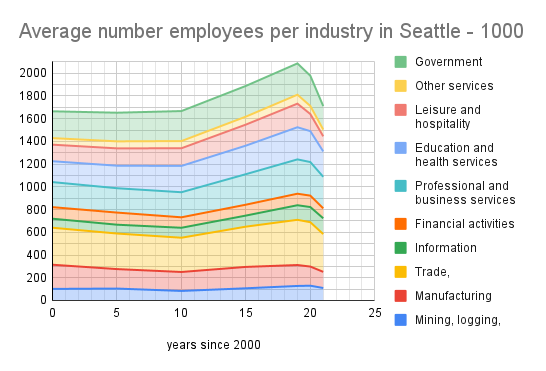
\includegraphics[width=\linewidth]{images/7D79AA67-B877-434A-BE22-808AC2C091B1.png}
                  \caption{stacked chart of $N_{I,C}(t)$ vs $t$ }
                  \label{fig:chart1}
                \end{figure}
                
            As can be seen, the workforce population which is the total height of \ref{fig:chart1} varies with time as expected.
            Plotting $P_{I,C}(t)$ vs $t$ we see: 
            \begin{figure}[H]
                  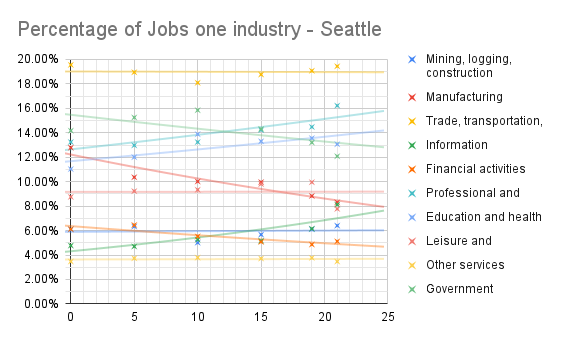
\includegraphics[width=\linewidth]{images/D111796A-6172-47DA-A494-CF6D7A966055.png}
                  \caption{stacked chart of $P_{I,C}(t)$ vs $t$ }
                  \label{fig:chart2}
                \end{figure}
                
                We saw that by Plotting $P_{I,C}(t)$ we see a clearer trend. We also do not need to account for change in population anymore using this method as $P_{I,C}(t)$ is a percentage of the total workforce population. In addition, we removed the data for 2020 as it seemed anomalous for every industry and so we thought it wasn't representative.
                
                
                
            \subsubsection{Exponential model}
            
                % All figures and graphs should have a title, a label, a caption, and the axes should be labelled.
                
                %h (here) – same location
                %t (top) – top of page
                %b (bottom) – bottom of page
                %p (page) – on an extra page
                %! (override) – will force the specified location
                %(\usepackage{float}) allows to set the option to [H], which is even stricter than [h!].
                The next task was to find the function: $P_{I,C}(t)$ in the form:
                \begin{equation}
                P_{I,C}(t) = a \cdot e^{bt}
                \end{equation}
                We are assuming that the proportion of an industry in a city varies as an exponential due to the following reasons: 
                \begin{itemize}
                    \item An exponential model more accurately represent changes in populations and natural growth over time
                    \item An exponential model better fits the data
                    \item An exponential model demonstrates asymptotic behaviour, not allowing for the percentage to fall below a certain level. This is closer to real life as industries will not shrink infinitely to 0. 
                \end{itemize}
                Using exponential regression, we were able to draw an exponential line of best fit for each $P_{I,C}(t)$. 
                
                \subsubsection{The $H_{I}$ constant}
                The Estimated percentage of jobs that can be done at home by occupation category in D3 was the basis for finding a value for $H_{I}$. Although it was not as straight forward as the industries named in D3, were not named the same as the industries in D1, which was the basis for our model of $P_{I,C}(t)$.
                
                So we tried to match each industry in D1 to 1 or more industries in D3. 
                
                We then calculated a value for $H_I$ for every industry in D1 based on the The Estimated percentage of jobs that can be done at home by occupation category in D3. If there are multiple matches we will calculate a weighted average based on the proportion of the certain occupation in the industry for $H_I$.
                
                \begin{tabular}{|p{4.5cm}|c|c|c|} % Defines where vertical lines appear and the column alignment left centre or right
                      \toprule 
                       \textbf{Industry in D1} & \textbf{Industry in D3}  & \textbf{weights} & \textbf{$H_I$}\\
                      \midrule 
                       Mining, logging, construction& Trade, transportation, and utilities & - & 0\%\\
                       Manufacturing& Production & - & 1\%\\
                       Trade, transportation, and utilities& Transportation and material moving & - & 30\%\\
                       Information& Computer and mathematical & - & 100\%\\
                       Financial activities& Business and financial operations & - & 88\%\\
                       Professional and business services & sales-office and administrative-management & 0.5-0.4-0.1 & 49\%\\
                       Education and health services& Education - health services&0.3-0.7 & 34\%\\
                       Leisure and hospitality& Food preparation and service related&- & 0\%\\
                       Other services & - & - & 50\%\\
                       Government & Legal-Office and administrative-Management& 0.2-0.7-0.1 & 74\%\\
                       
                       
                       

                      \bottomrule 
                    \end{tabular}
                
                Health and Education weights sourced from: \cite{eduStats} \cite{eduStats2}.
                
                % (USE THE REF AND LABEL COMMANDS because then figure numbers never go wrong)
                
                

        \subsection{Applying the Model (Results)}  
            % Considering any situations given to us in the question
            % And if none are given, make up some input data into the Model
            As we have 5 cities and 10 industries, we have 50 $P_{I,C}(t)$ functions. In the interest of saving space, I will give one example of this function:
            \begin{align}
            P_{trade,Omaha}(t) &= 0.237e^{-0.0117t} \\
            P_{trade,Omaha}(24) &= 17.90\% \\
            P_{trade,Omaha}(27) &= 17.28\% 
            \end{align}
            \begin{figure}[H]
                  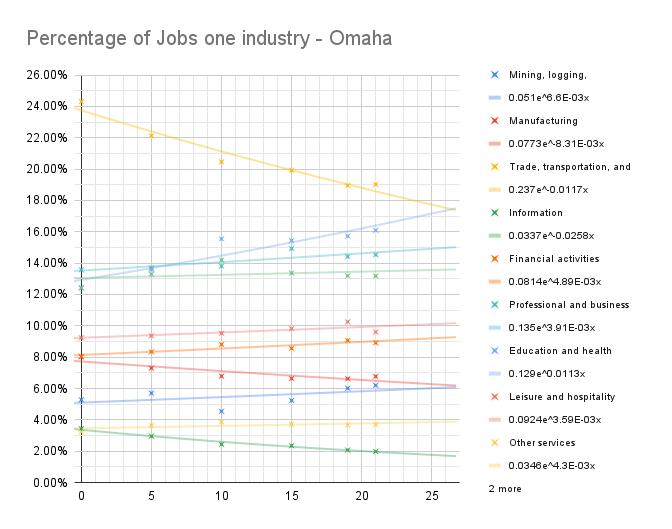
\includegraphics[width=\linewidth]{images/BEAB97A6-07C9-45F9-8B49-E371557909FE.png}
                  \caption{$P_{I,C}(t)$ vs $t$ with exponential trend line}
                  \label{fig:chart3}
                \end{figure}
                
            Finally we can find the percentage of "work from home ready" jobs by multiplying the $P_{I,C}(t)$ function by its corresponding $H_I$ value, and summing the results together to get a percentage of all the "work from home ready" jobs as a proportion of all the jobs in the city: $\Sigma P_{I,C}(t)\cdot H_I$ for all industries in the city.
                
            
            
                 \begin{tabular}{|c|c|c|} % Defines where vertical lines appear and the column alignment left centre or right
                      \toprule 
                       \textbf{City} & \textbf{year 2024}  & \textbf{year 2027} \\
                      \midrule 
                       Seattle & 41.31\% & 41.80\% \\
                       Omaha & 40.22\% & 40.36\% \\
                       Scranton & 35.91\% & 36.16\% \\
                       Liverpool & 31.22\% & 31.04\% \\
                       Barry & 39.07\% & 38.95\% \\
                       
                       
                       

                      \bottomrule 
                    \end{tabular}
                           
            
        \subsection{Implications}
            % What do the results mean?
            Our results show that approximately 40\% of jobs will be "work from home ready". This is not too different from the current rate. This is because we have assumed technology will not change much in the next 5 years to create a considerable change in the proportion of jobs that can be done from home.
            
        \subsection{Evaluating the Model}
            \subsubsection{Validation: Testing for Accuracy}
                % How accurate are the results? Can we use a separate dataset for which we have the "right answer" to check?
                To validate our data we looked online to other predictions for the percentage of jobs that could be done online. one of the pieces of data we came across was a Forbes article \cite{Forbes} that stated that it was about 37\%.And as working from home becomes easier as tech is more integrated into work I would say that our model accurately predicts the proportion of people able to work from home
                
            \subsubsection{Sensitivity Analysis: Testing for Stability and Sensitivity to Assumptions}
                % Sensitivity analysis can be done by taking constants and varying them by +/- n%; use a table for this perhaps.
                % discussion of how the model can be tested for accuracy, stability, and sensitivity to assumptions.
                % Think about what real world factors could lead to changes to a certain parameter value, and then address the effects of those changes on the model.  
                As an example of how sensitive the model is we will use the function $P_{trade,Omaha}(25)$ 
                where $P_{trade,Omaha}(t)&= 0.237e^{-0.0117t}$
                
                \begin{table}[h!]
                  \begin{center}
                    \label{tab:variables1} % Use this to create a label for the table so you can later reference it with \ref
                    \begin{tabular}{|c|c|} % Defines where vertical lines appear and the column alignment left centre or right
                      \toprule 
                       \textbf{$\Delta$ Time} & \textbf{ $P_{trade,Omaha}$} \\
                      \midrule 
                       +5\%  & +0.004\%\\ 
                       -5\% & -0.003\%\\
                      \bottomrule 
                    \end{tabular}
                    \caption{Sensitivity Analysis for Model $P_{trade,Omaha}$} 
                  \end{center}
                \end{table}
            \subsubsection{Model Strengths}
            preserves the impact of decreasing industries\\
            reflects the increasing dominance of certain industries\\
            not sensitive to small changes in time \\
            includes the population of the workforce \\
            uses the changing the pattern of industries in the model\\
        
    
            

            
            \subsubsection{Model Weaknesses}
            Over a very large periods of time (100+years) the model will become unsuitable as there is no way to conceivably predict the market share of each industry.\\
            
 %To write the report for problem1, write it in the problem1.tex file
      
    \section{Part II: Remote Control}
            
        \subsection{Problem Statement}
        In this part of the problem we are asked to "create a model that predicts whether an individual worker whose job is remote-ready will be allowed to and will choose to work from home".\\ \\ We take this to mean "given the characteristics of an individual worker such as their age, income, and family status, determine the probability that a worker with these characteristics will be allowed to \textit{and} want to from home, versus in the office. Then, compare this probability to a threshold value to give the binary answer of yes the worker will work from home or no they won't." \\ \\ This problem definition is advantageous because it scales more easily to larger numbers of people with the same characteristics, which will be needed when this model is reused in Q3. As human choices are not deterministic, a level of stochasticity can be employed if we use the probabilities, meaning not everyone with the same characteristics behaves in the same way.

        \subsection{Assumptions and Justifications}
            \begin{enumerate}[label={2.\arabic*.}]
                % All assumptions made in the model must be stated and justified. Do this in the following way:
                % \item creates a new bullet point for the new assumption
                % \assume{The thing you are assuming}{The justification for this assumption}
                % So overall write this: \item \assume{assumption}{justification}
                \item \label{independence} \assume{Whether a worker wants to work from home can be treated as independent of whether they are allowed to, and are in a remote ready job.}{This is a logical assumption because it is plausible to want to work from home but not be allowed to, to want to work from home and be allowed to, to not want to work from home and not be allowed to, and to not want to work from home and not be allowed to. In a purely theoretical sense, workers can make a decision on what they want to do separately from what they are allowed to do.}
                \item \label{representative} \assume{2019 ONS Data \cite{ONS2} for the proportion of workers of different ethnicities, sexes, professions etc. is representative of the pre-pandemic probability that a worker of the given ethnicity/sex etc. will work from home.}{The data was collected with a large sample size by a substantial public statistics organisation so it is reasonable to suppose this is the case. We use the most recent pre-pandemic data as this is likely to be the most representative.}
                \item \assume{We can account for the impact of the pandemic on working from home by applying a pandemic constant correction factor.}{This reflects how attitudes have changed toward remote working over the course of the pandemic. It would be preferred to determine this on the level of an individual but this requires data we don't currently have access to. See Extending the Model}
                \item \assume{The maximum age of a working person is 80 years and the minimum age is 20 years.}{This is probably an overestimate but should definitely not be an underestimate, which is important for our model to avoid negative age multipliers.}
                \item \assume{Working age is (apart from the above constraints), normally distributed with mean 35 and standard deviation 10}{This is likely because we would expect ages to be roughly symmetrical as there are factors which would both prevent younger workers getting into the labour market (education) and remove older workers (retirement). As we don't know the distribution and in the interests of time we make this assumption. By the 68–95–99.7 rule these parameter choices give us 99.7\% of the data within the stated min/max, meaning artificially rounding values into this range has next to no effect.} 
            \end{enumerate}
      
             
        \subsection{Analysing the Problem}  \label{analysis}
           It is insightful to represent the problem in probability notation.
            For a given worker, we define the following events.
            \begin{itemize}
                \item $W$, the event that the worker wants to work from home.
                \item $R$, the event that the worker's job enables them to work from home (remote ready job).
                \item $A$, the event that the worker's employer allows them to work from home. 
                \item $W_p$, the event that the worker wants to work from home pre-pandemic.
            \end{itemize}           
            We also define a pandemic correction $c$ for the worker which is a multiplying factor so that:
            \begin{equation}
                P(W) = \min{(1,c \cdot P(W_p))}
            \end{equation}
            This is designed to reflect how the pandemic has changed attitudes towards remote working. 
            
            With these events, what the question is asking for becomes clear:
            \begin{equation}
                P((W \cap A) | R) \equiv \frac{P(W \cap A \cap R)}{P(R)}
            \end{equation}
           \textit{To simplify the notation we omit conditioning on all of the features of the worker, as we can determine the probabilities of events derived from W, A, R from the worker's features.}\\
           
           Under Assumption \ref{independence} we can perform the following manipulation:
            \begin{equation}
                P((W \cap A) | R) \equiv \frac{P(W)\cdot P(A \cap R)}{P(R)} \equiv  \frac{c\cdot P(W_p)\cdot P(A \cap R)}{P(R)} \equiv  \frac{c\cdot P(W_p \cap A \cap R)}{P(R)}
            \end{equation}           
            
        \subsection{Defining Variables \& Constant Parameters} % To use an & or % you must put a \ before it or it is interpreted as a command.
            \subsubsection{Identifying Factors which affect the Outcome}
                %Explain here which variables/constants you thought were important when modelling this part of the problem and why they are important, how you came about identifying them and their values, and which ones you discarded or didn't include and why.
                % Detailed description of them and justification for why they are included (can use bps - itemize)
                
                When it comes to determining which workers work from home, the following factors were considered to be important. These were then condensed into variables for the model below.
                
                \begin{itemize}
                    \item \assume{Age}{The age of a worker will affect how "tech-savvy" they are, and remote working requires advanced use of digital technology, and also it will affect how much of an active social life the worker has.}
                    \item \assume{Commute Time}{In \cite{ONS}, the authors determine that "work-life balance was the greatest positive" of home working, and time spent commuting is reduced by home working, which affects work-life balance.}
                    \item \assume{House Features}{Working from home is dependent on whether or not a given worker has the space at home to concentrate and work.}
                    \item \assume{Income}{Working from home requires less transport costs which saves money, but infrastructure such as a good broadband connection is required.}
                    \item \assume{Sex}{This may affect the activities the way in which the person socialises with work colleagues, which could be an incentive to come into the office.}
                    \item \assume{Industry}{This affects their potential productivity when working from home, which may decide whether they are allowed to work from home.}
                    
                \end{itemize}
                
                The following features were discounted for the given reasons:
                \begin{itemize}
                    \item \assume{Family Characteristics}{Workers with young children may need to work from home to look after them, or alternatively may be distracted by them and want to work in the office. It was deemed not worth the time to investigate which of these is most likely. It can also be argued that the worker should not have to see their children if they are working from home; they may use a childminder.}   
                    \item \assume{Income}{Unfortunately we didn't have the required data to perform the below analysis for income as well as the factors used.}
                    \item \assume{Size of Team - how many others are working from home?}{It is important to maintain a workplace culture so for large organisations some staff may be required to come into the office, while for small businesses working from home may be preferred to cut costs. However the data was not available so this feature had to be discarded}
                \end{itemize}                
                
            \subsubsection{Table of Variables/Constants}
                % To summarise all of the choices made.
                % All tables should have a title, a header, a label, and a caption.
                \begin{table}[H]
                  \begin{center}
                    \label{tab:variables2} % Use this to create a label for the table so you can later reference it with \ref
                    \begin{tabular}{|c|c|p{6cm}|p{6cm}|c|} % Defines where vertical lines appear and the column alignment left centre or right
                      \toprule 
                       \textbf{Type} & \textbf{Symbol} & \textbf{Definition} & \textbf{Value} & \textbf{Units} \\
                      \midrule 
                       Constant & \(\sigma\) & Age standard deviation & 10 & years  \\ % & used to separate cells in a row; \\ used to separate rows.
                      \midrule 
                       Constant & \(\mu\) & Age mean & 35 & years  \\ % & used to separate cells in a row; \\ used to separate rows.
                      \midrule 
                       Variable & \(A\) & Age of a given worker & $20 < A < 80$ & years  \\ % & used to separate cells in a row; \\ used to separate rows.
                      \midrule 
                       Variable & \(S\) & Sex of a given worker & Male/Female & years  \\ % & used to separate cells in a row; \\ used to separate rows.
                      \midrule 
                       Variable & \(E\) & Ethnicity of a given worker & White/Mixed/Black/Asian/Other & None  \\ % & used to separate cells in a row; \\ used to separate rows.
                      \midrule 
                       Variable & \(I\) & Industry in which a given worker works & Selected from the ONS Standard Industrial Classification (SIC) Grouping \cite{ONSGroup} & None  \\ % & used to separate cells in a row; \\ used to separate rows.
                      \midrule 
                       Variable & \(L\) & Level of education of a given worker & No Qualification, GCSE, A Level, etc. American and British qualifications converted to standardise as necessary. & None  \\ % & used to separate cells in a row; \\ used to separate rows.
                      \midrule 
                       Variable & \(T\) & Time a worker works & Part Time or Full time & None  \\ % & used to separate cells in a row; \\ used to separate rows.
                      \midrule 
                       Variable & \(C\) & Commute Length of a given worker & 0 to 10000 & m  \\ % & used to separate cells in a row; \\ used to separate rows. 
                      \midrule 
                       Variable & \(H\) & Whether their house allows work from home or not. i.e. do they have a quiet place to work, based on average house sizes in the region & True/False & None\\
                      \midrule 
                       Constant & \(c\) & Pandemic WFH attitudes correction. We choose this value because data from \cite{VOXEU} figure 3 suggests that (cancelling out the hugely improved and worsened reactions) the average tolerance of working from home increased by 40\% during the pandemic. & 1.4 & None\\
                      \bottomrule 
                    \end{tabular}
                    \caption{Summary of Problem 2 Variables \& Constant Parameters}                
                  \end{center}
                \end{table}
            
 
        \subsection{Developing the Model}  
            %Describe mathematical approaches and..
            %..Justify modelling used, including the use of technical computing. Why does it make sense?
            % Motivate and fully explain the use of any complicated mathematical expressions.
            % Teams should justify the use of technical computing. That is, it must be clear why the team leveraged a computer program instead of just a calculator
            % Teams should include a summary of the purpose and key features of their code. 
            % If an outside library or method is used in a black-box way, it should be clear that the team understands the method’s functionality, and can justify why it was chosen. 

            %%*******REALLY IMPORTANT TO JUSTIFY THE MODELLING USED - why are you choosing each method?


            From the section \ref{analysis}, we identify that in order to get the output answer we need to obtain $P(R)$ and $P(W_p \cap A \cap R)$. $c$ was set as 1.4 as explained above.
           \begin{itemize}
               \item $P(R)$ can simply be determined based on the worker's industry using the given data in D3 \cite{given_data}. This tells us the proportion of jobs in a given industry being remote-ready. We could also use the model from Part I here however we decided not to as that brings in the additional complexity of the city the worker comes from. This should only be brought in at Part III and not Part II.
               \item $P(W_p \cap A \cap R)$ is the overall probability that this worker worked from home pre-pandemic (as a worker works from home if and only if they want to, are allowed to and can). We can determine this based on historical work-from-home data for the UK from the ONS \cite{ONS2}. This is the backbone of the model is the determination of $P(W_p \cap A \cap R)$. 
           \end{itemize}
           
           The ONS data \cite{ONS2} is provided in the following format. We convert this into a Python dictionary format, enabling easier processing.
            \begin{figure}[H]
              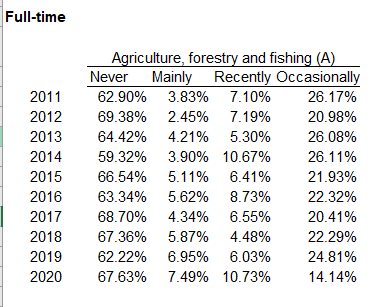
\includegraphics[width=200px]{exampleONSTable.png}
              \caption{An example data table from the ONS data. The 2019 data was extracted as it was the most recent, and converted into Python format for easy usage. See DataONS.py in the appendix.}
              \label{fig:ONSTable}
            \end{figure}
            
            The model created relies on technical computing through the use of object oriented programming to represent a person. We made this choice because it is easy and computationally cheap to spin up new instances of an OOP object, meaning it would work well when the model is reused in Part III for the Monte Carlo simulation.
            \\ \\
            The model works in the following way:
            \begin{enumerate}
                \item Determine the overall proportion of people actually working from home pre-pandemic, and call this the baseRate.
                \item For each of the persons's characteristics, such as their ethnicity, whether they work full time or part time etc we use ONS data to determine the percentage of people working from home within these categories.
                \item We then divide these by the base rate so that if a particular industry is "bang average", no change is made to the probability of working from home pre-pandemic, whereas if a given industry is more or less prone to working from home we multiply the baseRate probability by the factor industry rate over baseRate, for example.
                \item This process of multiplying the rate is repeated for each of a given person's characteristics.
                \item We then incorporate the continuous (non categoric) factors affecting working from home of commute distance and age. To incoporate commute distance we take the tanh of the commute distance in km and multiply it by the current probability of working from home for the person. This is justified because tanh goes through the origin, which means that if a person has 0 commute distance their chance of working from home becomes 0 because it is no extra effort to go into the office. As the person gets further away from the office (commute lengthens) the probability of working from home increases as they will not want to have to commute. We use tanh because it peaks at 1 meaning we can't increase the probability of working from home above 1, and once a worker gets far from their office an increase of 1km has less effect.
                \item To incorporate the age of the worker we again multiply the current probability by a new value, which in this case is defined as multiplying factor = $1.5-0.5 \cdot e^{\frac{A-20}{80}$. This yields the desired behaviour of a steady decline in likelihood of WFH with age; starting at 1 for a 20 year old due to level of tech saviness. 
            \end{enumerate}
            
        \subsection{Applying & Evaluating the Model (Results)}  
            % Considering any situations given to us in the question
            % And if none are given, make up some input data into the Model
            To evaluate the model we consider some example people. It's impossible to try all of the many intersections of the different factors but we think the following demonstrates a range of logical behaviours. The model's successful integration into Part III leading to reasonable results suggests it is good. See that section for more details.
            \begin{figure}[H] 
              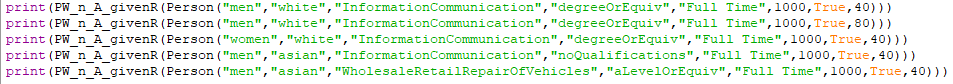
\includegraphics[width=200px]{testValues.png}
              \caption{Input to the model to apply and evaluate it}
              \label{fig:testValues}
            \end{figure}  
            \begin{figure}[H]
              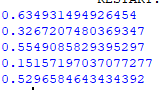
\includegraphics[width=200px]{testValuesOut.png}
              \caption{Probabilities of the respective people working from home.}
              \label{fig:testValuesOut}
            \end{figure}  
            
             %To write the report for problem2, write it in the problem2.tex file
        
    \section{Part III: Just a Little Home-work}
                % "The discriminator - many teams will do something, while only a few will have striking results"
    
    
        \subsection{Problem Statement}
        % State the problem and describe how you "redefined" it - and also maybe a single sentence before that on why it is important.
        In this section of the challenge, we are asked to "synthesize [our] models from the first two questions to create a model which, for a given city, estimates the percentage of workers who will work remotely." \\ \\
        This should work for 2024 and 2027 in the same cities considered previously, namely  Seattle, Omaha, Scranton, Liverpool, and Barry, and then be used to determine a relative ranking for the different cities of the impact of remote working on them. 
        
        \subsection{Assumptions and Justifications}
            \begin{enumerate}[label={3.\arabic*.}]
                % All assumptions made in the model must be stated and justified. Do this in the following way:
                % \item creates a new bullet point for the new assumption
                % \assume{The thing you are assuming}{The justification for this assumption}
                % So overall write this: \item \assume{assumption}{justification}

                \item \assume{There are no major changes to the population demographic between now and 2027}{It is reasonable to assume that there will not be any significant changes to the factors that affect the population demographic. This includes percentage of population that are of working age to be constant and there will be no net change in migration, as well as things like ethnicity and education levels as we have used current data to make predictions about these values for the future. This is reasonable as 2024 and 2027 are not that far away.}
                
                \item \assume{The impact of house size on working from home can be modelled as 90\% of people having the housing space and bandwidth to work from home.}{Due to a lack of time and consistent data we make this general assumption for all of the cities considered.}
                
                \item{Within each sex, for example, each ethnicity is distributed in the same way as it is for the whole population. i.e. ethnicity and sex and the other ways the population is to be divided are independent.}{This is a reasonable assumption to make because we don't have a breakdown of the individual characteristics of each person. As we generate a large random population the impact of this evens out.}

            \end{enumerate}
     
             
        \subsection{Analysing the Problem}  
            It is valuable to take a moment to understand the characteristics of what we have developed so far and what we need for this part. While Part I of the problem studies, on the level of cities and their industries, the proportion of jobs being "work from home ready", Part II asks on the individual level whether someone who can work from home will do so. \\ \\ For Part III we require a model which will, on the city level, determine the proportion of people who will actually work from home. Hence this leads us to the plan of using a simple agent-based model to combine the individual and whole city characteristics. We will use results from Part I to identify the number of people in each industry in each city in 2024 and 2027, then use a Monte Carlo simulation to create a profile for each member of the population of each city. Each profile can be run through the model from Part II to produce a probability of the given person working from home, and using a random variable we can count them in or out. Then summing for the whole population allows us to obtain percentages. 
            
        \subsection{Defining Variables \& Constant Parameters} 
            \subsubsection{Identifying Variables and Determining Constant Values}
                %Explain here which variables/constants you thought were important when modelling this part of the problem and why they are important, how you came about identifying them and their values, and which ones you discarded or didn't include and why.
                % Detailed description of them and justification for why they are included (can use bps - itemize)
                As we rely on the model from section 2 to identify the work from home preferences of a given individual, we use the same input data to as we used there for each person. 
                
            \subsubsection{Table of Variables/Constants}
                % To summarise all of the choices made.
                % All tables should have a title, a header, a label, and a caption.
                \begin{table}[h!]
                  \begin{center}
                    \label{tab:variables3} % Use this to create a label for the table so you can later reference it with \ref
                    \begin{tabular}{|c|c|p{5cm}|c|c|} % Defines where vertical lines appear and the column alignment left centre or right
                      \toprule 
                       \textbf{Type} & \textbf{Symbol} & \textbf{Definition} & \textbf{Value} & \textbf{Units} \\
                      \midrule 
                      Variable & $N_{I,C,T}$ & The number of people in industry I in city C at time T. As in Part I & - & 1000 people  \\ % & used to separate cells in a row; \\ used to separate rows.
                      \bottomrule 
                    \end{tabular}
                    \caption{Summary of Problem 3 Variables \& Constant Parameters}                
                  \end{center}
                \end{table}
            

            
        \subsection{Developing the Model}  
            %Describe mathematical approaches and..
            %..Justify modelling used, including the use of technical computing. Why does it make sense?
            % Motivate and fully explain the use of any complicated mathematical expressions.
            % Teams should justify the use of technical computing. That is, it must be clear why the team leveraged a computer program instead of just a calculator
            % Teams should include a summary of the purpose and key features of their code. 
            % If an outside library or method is used in a black-box way, it should be clear that the team understands the method’s functionality, and can justify why it was chosen. 

            %%*******REALLY IMPORTANT TO JUSTIFY THE MODELLING USED - why are you choosing each method?
            
            We use a Monte Carlo simulation in which we determine the expected population in 2024 and 2027 of each of the cities investigated. For each member of the population, we generate a Person object so that overall the characteristics of the employees match the summary statistics for the town. This generation is performed with the recursiveGen algorithm, which takes a number of people it must generate, a city, and a year. It splits the population in half for each sex, then calls itself to split each of these groups into sections for ethnicity based on the relevant city's ethnicity percentages and so on for all of the other factors. At the base case, it has generated a value for all of the attributes of the Person class so it instantiates a number of Person objects equal to amount. It calls the Part II model on these people and sums the results to give a total number of people working from home in 2024 and 2027 for each city. This is then converted to a percentage in each case.
        

        \subsection{Applying the Model (Results)}  
            % Considering any situations given to us in the question
            % And if none are given, make up some input data into the Model

            Using this model we achieve the following results for the percentage of people working from home:
                \begin{table}[h!]
                  \begin{center}
                    \label{tab:resultsFinal} % Use this to create a label for the table so you can later reference it with \ref
                    \begin{tabular}{|c|c|c|c|c|} % Defines where vertical lines appear and the column alignment left centre or right
                      \toprule 
                       \textbf{Result Year} & \textbf{2024 predictions} & \textbf{2024 ranking} & \textbf{2027 predictions} & \textbf{2027 ranking} \\
                      \midrule 
                      Barry & 26.51\% & 4th & 26.59\% & 5th  \\
                      Liverpool & 27.37\% & 3rd & 29.13\% & 3rd  \\
                      Omaha & 29.07\% & 2nd & 29.26\% & 2nd  \\
                      Seattle & 30.73\% & 1st & 32.45\% & 1st  \\
                      Scranton & 26.36\% & 5th & 26.63\% & 4th  \\
                        
                      \bottomrule 
                    \end{tabular}
                    \caption{Summary of Problem 3 Results for 2024 \& 2027}                
                  \end{center}
                \end{table}
                
            As is to be expected, the most technological city on Earth is to be most revolutionised by remote working, while a small town in Wales where the main industries have always been mining and fishing \cite{barryStory} serves less to benefit. This suggests that as a country if we desire fairness and equality of opportunity we should invest more in remote working capacity for smaller towns like Barry.
            
        \subsection{Evaluating the Model}
            
            \subsubsection{Validation: Testing for Accuracy}
                % How accurate are the results? Can we use a separate dataset for which we have the "right answer" to check?
                The model returns a plausible result. The latest ONS figures suggest that 30\% of working adults work from home either partially or exclusively \cite{ONS3}. A modest increase on pre-pandemic levels is to be expected.
            
            \subsubsection{Sensitivity Analysis: Testing for Stability and Sensitivity to Assumptions}
                % Sensitivity analysis can be done by taking constants and varying them by +/- n%; use a table for this perhaps.
                % discussion of how the model can be tested for accuracy, stability, and sensitivity to assumptions.
                % Think about what real world factors could lead to changes to a certain parameter value, and then address the effects of those changes on the model.           
                % Remember that you can reference previously defined assumptions with the \label (on defining) and \ref (to reference) commands. 
                Due to time constraints we could only perform this analysis on 2024 results
                \begin{table}[h!]
                  \begin{center}
                    \label{tab:variables1} % Use this to create a label for the table so you can later reference it with \ref
                    \begin{tabular}{|p{4cm}|c|c|c|c|c|c|} % Defines where vertical lines appear and the column alignment left centre or right
                      \toprule 
                       \textbf{$\Delta$ Pandemic Correction Constant} & \textbf{Barry} & \textbf{Liverpool} & \textbf{Omaha} & \textbf{Seattle} & \textbf{Scranton}& \textbf{Average}\\
                      \midrule 
                      +10\% & +9.7\% & +9.8\% & +9.9\% & +9.8\% & +9.7\% & +9.78\%\\
                       +5\%  & +4.5\% & +4.9\% & +4.9\% & +4.8\% & +4.6\% & +4.74\% \\ 
                       -5\% & -4.8\% & -4.7\% & -5.0\% & -4.7\% & -5.1\% & -4.86\%\\
                       -10\% & -9.7\% & -10.0\% & -9.9\% & -9.9\% & -9.9\% & -9.88\%\\
                      \bottomrule 
                    \end{tabular}
                    \caption{Sensitivity Analysis for Model 3} 
                  \end{center}
                \end{table}
                It is desirable for the impact of changing model assumptions to be as low as possible so that if they are wrong, the model is not rendered useless. The most obvious assumption made here was the choice of 1.4 for the pandemic correction constant. We see that varying this changes the percentage of people working from home in the expected way, with change magnitude always less than or equal to the change in the constant $c$ which is good.
                
    
            \subsubsection{Model Strengths}
                The model inputs a wide range of factors including population and job demographics which means the model can be used for any city with such data values, Furthermore all predicted results are between 26\% and 34\% which is similar to current levels and significantly above pre-pandemic levels.
            \subsubsection{Model Weaknesses}
                The main weakness of the model is that it is complicated and requires a lot of data about each of the places. It was time consuming to format all of this data for each place and sector correctly for the program, so extending the model to other places would be painful.
            
        \subsection{Extending the Model}
            % Further research that could be performed if we had extra time
            % Creativity, good work, and acknowledging where you fall short and what you would have done with more time is valued. The judges are particularly interested in each team’s approach and methods.
            
            If we had more time we would:
            \begin{itemize}
                \item Perform greater validation on this model to ensure that it is accurate, by removing and varying other assumptions and parameters to identify the impact.
                \item Simplify the model or factor out some of the data so it can be more easily extended to other cities.
            \end{itemize}
        
         %To write the report for problem3, write it in the problem3.tex file
        
    \section{Joining the Dots: Conclusions}
        %   Team made connections between all three parts and the overall driving question.
        %   Analyses results, discusses model strengths, weaknesses and areas which can be improved
    
       In this paper, we investigated how trends towards homeworking can be applied into the future, in a post pandemic society. In Part I of the problem, we are asked to determined the percentage of jobs that can work remotely in the 5 given cities, achieving results of around 40\% of jobs being able to be completed remotely in each city, which is consistent with other data. In Part II, we identified for a given worker who can work from home, whether they will actually work from home, considering the likelihood that they want to work from home and that they are allowed to work remotely. For example, we gave a white male IT Worker aged 40 63\% chance of working from home, for example. In Part III a fusion of the models for jobs (Part I) and for individuals (Part II) in the form of a Monte Carlo simulation was employed based on projected demographics of each town or city to obtain the expected proportion of remote workers. Results ranging from 26.5\% for Barry in 2024 32.5\% for Seattle in 2027 were logical.
       \\ \\
       As a result of our work, we make the policy recommendation for the Prime Minister that working from home will remain a substantial part of the UK and US work-forces. He must consider it in future labour policies, and the impact of improved technology on the propensity to work from home should be factored into his levelling up agenda. 
    \newpage
    \section{References} % To add a source, go to the main.bib file and copy the dummy entry and replace the field values with the appropriate values.
        \nocite{keyes_2021} % Sources that you refer to but you don't want to reference anywhere particular in the document - you need to use the \nocite command otherwise they WILL NOT appear in the bibliography
        \nocite{given_data} % if we cite elsewhere then remove this,.
        \begingroup
            \renewcommand{\section}[2]{} % Prevents double reference titles.
            \bibliography{main}
            \bibliographystyle{plain}            
        \endgroup
      
       % When citing outside sources, clearly explain what statistics, models, equations, or insights you took from each source.
    
    \newpage
    \section{Appendix: Code Listing for Technical Computing Consideration}
        % Ensure code is commented! 
        % "some code commenting, meaningful variable names, and appropriate use of functions and code-reuse will make it easier for judges to understand what a program is doing and how it contributes to the team's model."
        % EXPLAIN THE ALGORITHM INSIDE THE TEXT OF THE REPORT
        
        %Teams should justify the use of technical computing. That is, it must be clear why the team leveraged a computer program instead of just a calculator.
        %Teams should include a summary of the purpose and key features of their code.
        %If an outside library or method is used in a black-box way, it should be clear that the team understands the method’s functionality, and can justify why it was chosen.
        
        \subsection{Part II}
            \textbf{dataONS.py}
            \lstinputlisting{code/dataONS.py} %% Replace with actual code file name! Upload file into the code folder and then duplicate this command to paste your code in.
            \newpage
            \textbf{Question2.py}
            \lstinputlisting{code/Question2.py} %% Replace with actual code file name! Upload file into the code folder and then duplicate this command to paste your code in.
            
            \newpage
        \subsection{Part III}
            \textbf{Question3.py}
            \lstinputlisting{code/Question3.py} %% Replace with actual code file name! Upload file into the code folder and then duplicate this command to paste your code in.
        



\end{document}